% Figura del nodo: formulazione iniziale (§4.3). Compilare con: pdflatex nodi.tex
\documentclass[border=8pt]{standalone}
\usepackage[utf8]{inputenc}
\usepackage[T1]{fontenc}
\usepackage{lmodern}
\usepackage{amsmath,amssymb}
\usepackage{tikz}
\usetikzlibrary{arrows.meta,calc}
\renewcommand{\familydefault}{\sfdefault}
\definecolor{bl}{HTML}{2F6FD6}\definecolor{blf}{HTML}{DCE8FA}
\definecolor{orc}{HTML}{E8692B}\definecolor{orf}{HTML}{FBE3D6}
\definecolor{gr}{HTML}{9A9A9A}\definecolor{mid}{HTML}{666666}
\tikzset{
  dim/.style={{Latex[length=1.6mm]}-{Latex[length=1.6mm]},mid,thin},
  dimb/.style={{Latex[length=1.6mm]}-{Latex[length=1.6mm]},bl,semithick},
  dimo/.style={{Latex[length=1.6mm]}-{Latex[length=1.6mm]},orc,semithick},
  bfrect/.style={draw=bl,line width=1.1pt,fill=blf},
  flrect/.style={draw=orc,line width=1.1pt,fill=orf},
  prof/.style={gr,line width=1pt},
  ttl/.style={anchor=west,font=\bfseries\small},
  lab/.style={font=\footnotesize},
  note/.style={font=\scriptsize,text=mid},
}
\begin{document}
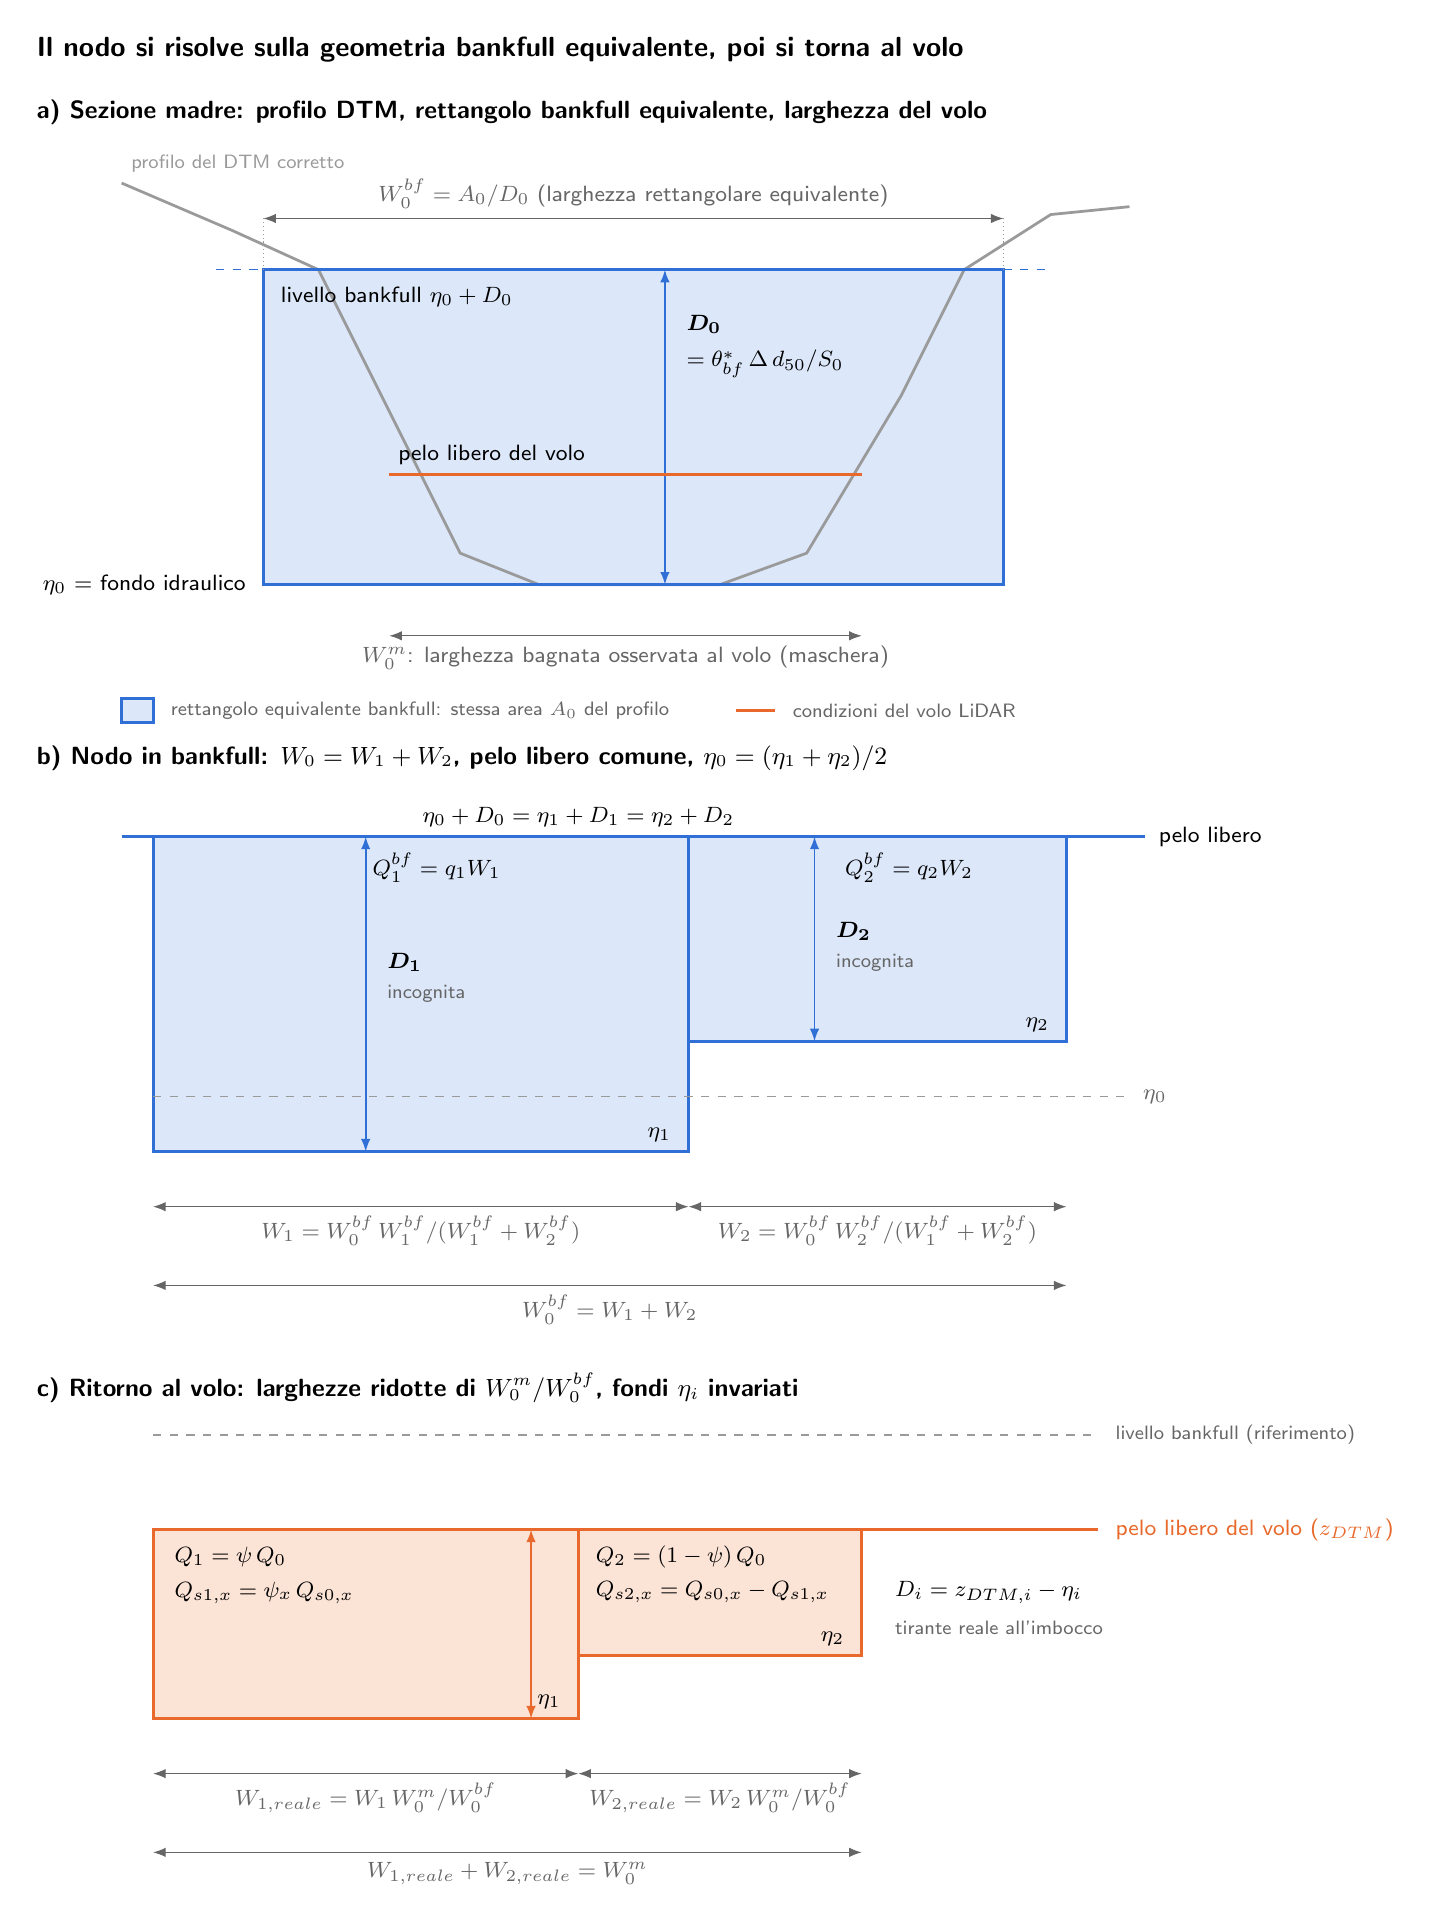
\begin{tikzpicture}[x=1cm,y=1cm]
\node[anchor=west,font=\bfseries\normalsize] at (0,0.6) {Il nodo si risolve sulla geometria bankfull equivalente, poi si torna al volo};
% ---------------- a ----------------
\node[ttl] at (0,-0.2) {a) Sezione madre: profilo DTM, rettangolo bankfull equivalente, larghezza del volo};
\begin{scope}[shift={(0,-6.4)}]
\node[note,text=gr,anchor=west] at (1.2,5.55) {profilo del DTM corretto};
\fill[blf] (3.0,0.2) rectangle (12.4,4.2);
\draw[prof] (1.2,5.3) -- (2.6,4.7) -- (3.7,4.2) -- (4.5,2.6) -- (5.5,0.6) -- (6.5,0.2) -- (8.8,0.2) -- (9.9,0.6) -- (11.1,2.6) -- (11.9,4.2) -- (13.0,4.9) -- (14,5.0);
\draw[bl,line width=1.1pt] (3.0,0.2) rectangle (12.4,4.2);
\draw[bl,dashed] (2.4,4.2) -- (3.0,4.2); \draw[bl,dashed] (12.4,4.2) -- (13.0,4.2);
\node[lab,anchor=north west] at (3.1,4.1) {livello bankfull $\eta_0+D_0$};
\draw[dimb] (8.1,0.2) -- (8.1,4.2);
\node[lab,anchor=west] at (8.25,3.5) {$\boldsymbol{D_0}$};
\node[lab,anchor=west] at (8.25,3.0) {$=\theta^{*}_{bf}\,\Delta\,d_{50}/S_0$};
\draw[orc,line width=1.3pt] (4.6,1.6) -- (10.6,1.6);
\node[lab,anchor=south] at (5.9,1.6) {pelo libero del volo};
\draw[dim] (3.0,4.85) -- (12.4,4.85) node[midway,above,lab] {$W_0^{bf}=A_0/D_0$ (larghezza rettangolare equivalente)};
\draw[gr,densely dotted] (3.0,4.2) -- (3.0,4.85); \draw[gr,densely dotted] (12.4,4.2) -- (12.4,4.85);
\node[lab,anchor=east] at (2.9,0.2) {$\eta_0$ = fondo idraulico};
\draw[dim] (4.6,-0.45) -- (10.6,-0.45) node[midway,below,lab] {$W_0^{m}$: larghezza bagnata osservata al volo (maschera)};
\draw[bfrect] (1.2,-1.55) rectangle (1.6,-1.25); \node[note,anchor=west] at (1.7,-1.4) {rettangolo equivalente bankfull: stessa area $A_0$ del profilo};
\draw[orc,line width=1.3pt] (9.0,-1.4) -- (9.5,-1.4); \node[note,anchor=west] at (9.6,-1.4) {condizioni del volo LiDAR};
\end{scope}
% ---------------- b ----------------
\node[ttl] at (0,-8.4) {b) Nodo in bankfull: $W_0=W_1+W_2$, pelo libero comune, $\eta_0=(\eta_1+\eta_2)/2$};
\begin{scope}[shift={(0,-14.0)}]
\draw[bl,line width=1pt] (1.2,4.6) -- (14.2,4.6); \node[lab,anchor=west] at (14.25,4.6) {pelo libero};
\node[lab,anchor=south] at (7.0,4.6) {$\eta_0+D_0=\eta_1+D_1=\eta_2+D_2$};
\draw[bfrect] (1.6,0.6) rectangle (8.4,4.6);
\draw[bfrect] (8.4,2.0) rectangle (13.2,4.6);
\draw[gr,dashed] (1.6,1.3) -- (14.0,1.3); \node[lab,text=mid,anchor=west] at (14.05,1.3) {$\eta_0$};
\node[lab] at (5.2,4.2) {$Q_1^{bf}=q_1W_1$}; \node[lab] at (11.2,4.2) {$Q_2^{bf}=q_2W_2$};
\draw[dimb] (4.3,0.6) -- (4.3,4.6); \node[lab,anchor=west] at (4.45,3.0) {$\boldsymbol{D_1}$}; \node[note,anchor=west] at (4.45,2.6) {incognita};
\draw[dimb] (10.0,2.0) -- (10.0,4.6); \node[lab,anchor=west] at (10.15,3.4) {$\boldsymbol{D_2}$}; \node[note,anchor=west] at (10.15,3.0) {incognita};
\node[lab,anchor=south east] at (8.3,0.6) {$\eta_1$}; \node[lab,anchor=south east] at (13.1,2.0) {$\eta_2$};
\draw[dim] (1.6,-0.1) -- (8.4,-0.1) node[midway,below,lab] {$W_1=W_0^{bf}\,W_1^{bf}/(W_1^{bf}+W_2^{bf})$};
\draw[dim] (8.4,-0.1) -- (13.2,-0.1) node[midway,below,lab] {$W_2=W_0^{bf}\,W_2^{bf}/(W_1^{bf}+W_2^{bf})$};
\draw[dim] (1.6,-1.1) -- (13.2,-1.1) node[midway,below,lab] {$W_0^{bf}=W_1+W_2$};
\end{scope}
% ---------------- c ----------------
\node[ttl] at (0,-16.4) {c) Ritorno al volo: larghezze ridotte di $W_0^{m}/W_0^{bf}$, fondi $\eta_i$ invariati};
\begin{scope}[shift={(0,-21.6)}]
\draw[gr,dashed] (1.6,4.6) -- (13.6,4.6); \node[note,anchor=west] at (13.7,4.6) {livello bankfull (riferimento)};
\draw[flrect] (1.6,1.0) rectangle (7.0,3.4);
\draw[flrect] (7.0,1.8) rectangle (10.6,3.4);
\draw[orc,line width=1.3pt] (1.6,3.4) -- (13.6,3.4); \node[lab,text=orc,anchor=west] at (13.7,3.4) {pelo libero del volo ($z_{DTM}$)};
\node[lab,anchor=west] at (1.75,3.05) {$Q_1=\psi\,Q_0$}; \node[lab,anchor=west] at (1.75,2.6) {$Q_{s1,x}=\psi_x\,Q_{s0,x}$};
\node[lab,anchor=west] at (7.1,3.05) {$Q_2=(1-\psi)\,Q_0$}; \node[lab,anchor=west] at (7.1,2.6) {$Q_{s2,x}=Q_{s0,x}-Q_{s1,x}$};
\draw[dimo] (6.4,1.0) -- (6.4,3.4); \node[lab,anchor=south east] at (6.9,1.0) {$\eta_1$}; \node[lab,anchor=south east] at (10.5,1.8) {$\eta_2$};
\node[lab,anchor=west] at (10.9,2.6) {$D_i=z_{DTM,i}-\eta_i$}; \node[note,anchor=west] at (10.9,2.15) {tirante reale all'imbocco};
\draw[dim] (1.6,0.3) -- (7.0,0.3) node[midway,below,lab] {$W_{1,reale}=W_1\,W_0^{m}/W_0^{bf}$};
\draw[dim] (7.0,0.3) -- (10.6,0.3) node[midway,below,lab] {$W_{2,reale}=W_2\,W_0^{m}/W_0^{bf}$};
\draw[dim] (1.6,-0.7) -- (10.6,-0.7) node[midway,below,lab] {$W_{1,reale}+W_{2,reale}=W_0^{m}$};
\end{scope}
\end{tikzpicture}
\end{document}
